\section{Images without a good run}
\label{sec:suppl-unsolved}
\Cref{fig:suppl-unsolved-ff,fig:suppl-unsolved-in} complete \cref{M-fig:unsolved}. It shows every FFHQ image on which FAST-DIPS produced no \good run in $64$ runs ($7$ of $180$), and the first $8$ of the $22$ ImageNet images (FAST-DIPS, $64$ runs on the first ImageNet image set) with no \good run in any orientation, ordered by the SHA-256 of the image id, a rule fixed before plotting.
For each image: the ground truth, the lowest-residual run as returned, and the best run over all runs and orientations (the orbit oracle), shown in its best orientation.
PSNR is computed against the ground truth; \good needs $25$\,dB on FFHQ and $20$\,dB on ImageNet.
\begin{itemize}[leftmargin=*,itemsep=1pt,topsep=2pt]
\item \textbf{FFHQ.} Five of the seven are near misses: their best run reaches $22.8$--$24.7$\,dB and is hard to tell from the ground truth at this size. One reaches $20.1$\,dB, and its lowest-residual run is rotated ($6.8$\,dB). One fails outright ($15.3$\,dB). For six of the seven, the lowest-residual run is within $0.4$\,dB of the best.
\item \textbf{ImageNet.} The best run reaches $12.2$--$19.8$\,dB, and the images are visibly wrong. For three of the eight, the best run is a rotated one.
\end{itemize}
These are the images that the coverage curves of \cref{M-sec:selection} count and that ground-truth best-of-$K$ numbers hide.

\begin{figure}[p]
\centering\scriptsize
\setlength{\tabcolsep}{0.8pt}\renewcommand{\arraystretch}{0.8}
\begin{tabular}{@{}cccccc@{}}
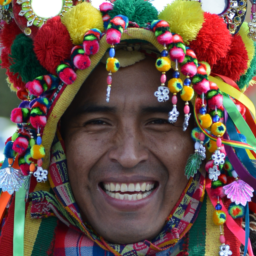
\includegraphics[width=0.158\textwidth]{../fig/unsolved/FAST_never_good_01_ref.png} & 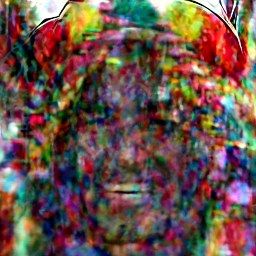
\includegraphics[width=0.158\textwidth]{../fig/unsolved/FAST_never_good_01_e0.png} & 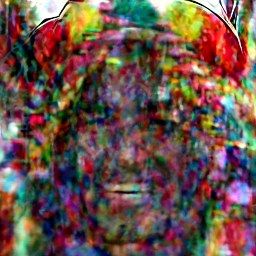
\includegraphics[width=0.158\textwidth]{../fig/unsolved/FAST_never_good_01_orc.png} & 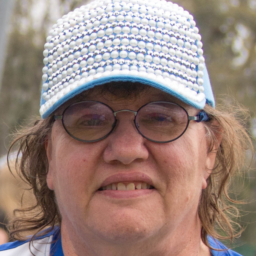
\includegraphics[width=0.158\textwidth]{../fig/unsolved/FAST_never_good_02_ref.png} & 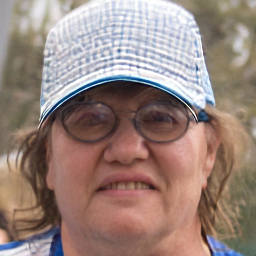
\includegraphics[width=0.158\textwidth]{../fig/unsolved/FAST_never_good_02_e0.png} & 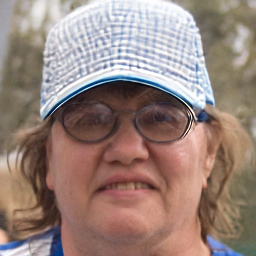
\includegraphics[width=0.158\textwidth]{../fig/unsolved/FAST_never_good_02_orc.png} \\
ground truth & lowest residual, 15.3\,dB & best, 15.3\,dB & ground truth & lowest residual, 24.2\,dB & best, 24.2\,dB \\[3pt]
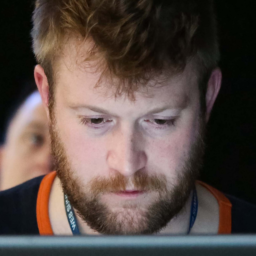
\includegraphics[width=0.158\textwidth]{../fig/unsolved/FAST_never_good_03_ref.png} & 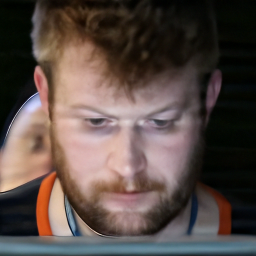
\includegraphics[width=0.158\textwidth]{../fig/unsolved/FAST_never_good_03_e0.png} & 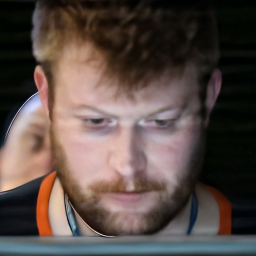
\includegraphics[width=0.158\textwidth]{../fig/unsolved/FAST_never_good_03_orc.png} & 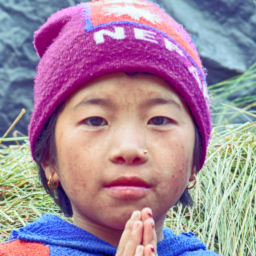
\includegraphics[width=0.158\textwidth]{../fig/unsolved/FAST_never_good_04_ref.png} & 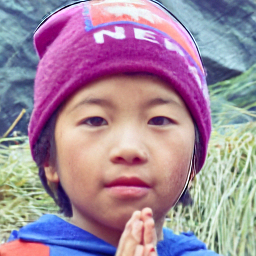
\includegraphics[width=0.158\textwidth]{../fig/unsolved/FAST_never_good_04_e0.png} & 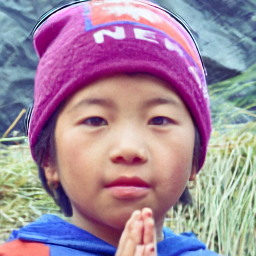
\includegraphics[width=0.158\textwidth]{../fig/unsolved/FAST_never_good_04_orc.png} \\
ground truth & lowest residual, 22.5\,dB & best, 22.8\,dB & ground truth & lowest residual, 24.5\,dB & best, 24.7\,dB \\[3pt]
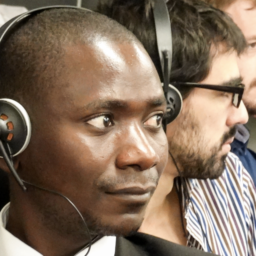
\includegraphics[width=0.158\textwidth]{../fig/unsolved/FAST_never_good_05_ref.png} & 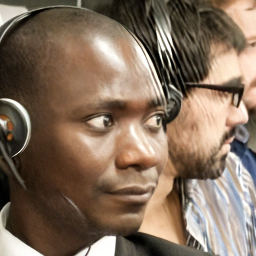
\includegraphics[width=0.158\textwidth]{../fig/unsolved/FAST_never_good_05_e0.png} & 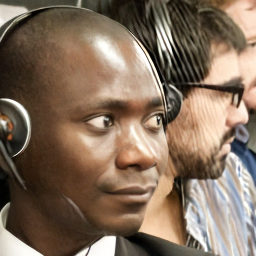
\includegraphics[width=0.158\textwidth]{../fig/unsolved/FAST_never_good_05_orc.png} & 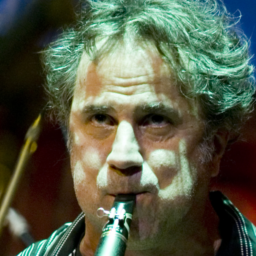
\includegraphics[width=0.158\textwidth]{../fig/unsolved/FAST_never_good_06_ref.png} & 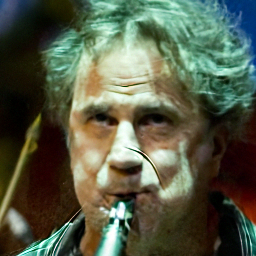
\includegraphics[width=0.158\textwidth]{../fig/unsolved/FAST_never_good_06_e0.png} & 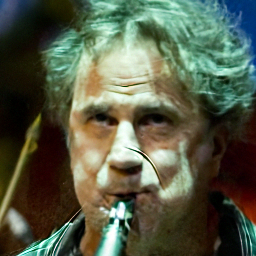
\includegraphics[width=0.158\textwidth]{../fig/unsolved/FAST_never_good_06_orc.png} \\
ground truth & lowest residual, 24.0\,dB & best, 24.1\,dB & ground truth & lowest residual, 24.2\,dB & best, 24.2\,dB \\[3pt]
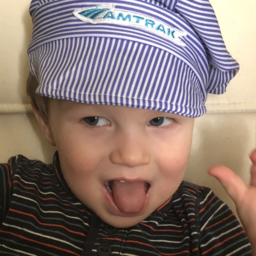
\includegraphics[width=0.158\textwidth]{../fig/unsolved/FAST_never_good_07_ref.png} & 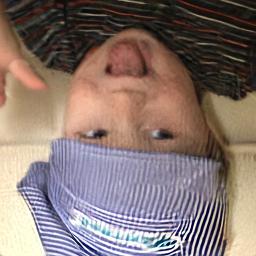
\includegraphics[width=0.158\textwidth]{../fig/unsolved/FAST_never_good_07_e0.png} & 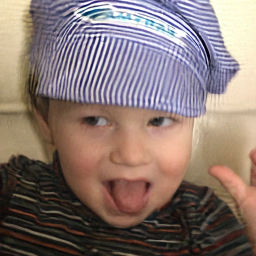
\includegraphics[width=0.158\textwidth]{../fig/unsolved/FAST_never_good_07_orc.png} &  &  &  \\
ground truth & lowest residual, 6.8\,dB & best, 20.1\,dB &  &  &  \\[3pt]
\end{tabular}
\caption{\textbf{FFHQ: all $7$ images on which FAST-DIPS produces no \good run in $64$ runs.} Each triple: ground truth, lowest-residual run as returned, best run over all runs and orientations (in its best orientation), with PSNR. Original $256\times256$ tiles.}
\label{fig:suppl-unsolved-ff}
\end{figure}

\begin{figure}[p]
\centering\scriptsize
\setlength{\tabcolsep}{0.8pt}\renewcommand{\arraystretch}{0.8}
\begin{tabular}{@{}cccccc@{}}
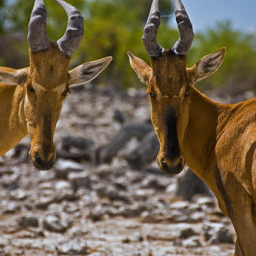
\includegraphics[width=0.158\textwidth]{../fig/unsolved/D4_never_orbit_01_ref.png} & 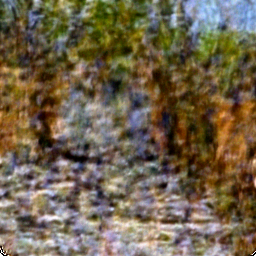
\includegraphics[width=0.158\textwidth]{../fig/unsolved/D4_never_orbit_01_e0.png} & 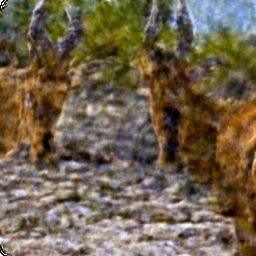
\includegraphics[width=0.158\textwidth]{../fig/unsolved/D4_never_orbit_01_orc.png} & 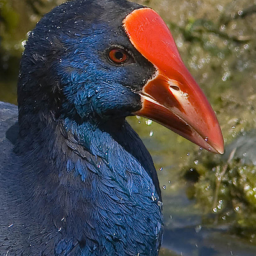
\includegraphics[width=0.158\textwidth]{../fig/unsolved/D4_never_orbit_02_ref.png} & 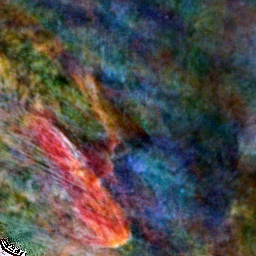
\includegraphics[width=0.158\textwidth]{../fig/unsolved/D4_never_orbit_02_e0.png} & 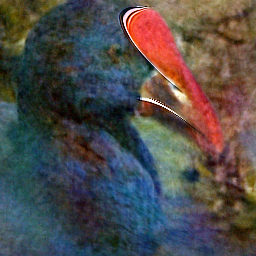
\includegraphics[width=0.158\textwidth]{../fig/unsolved/D4_never_orbit_02_orc.png} \\
ground truth & lowest residual, 17.3\,dB & best, 18.3\,dB & ground truth & lowest residual, 12.0\,dB & best, 19.8\,dB \\[3pt]
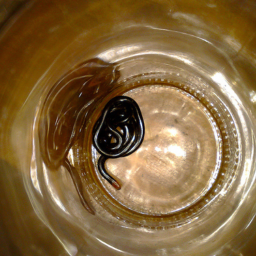
\includegraphics[width=0.158\textwidth]{../fig/unsolved/D4_never_orbit_03_ref.png} & 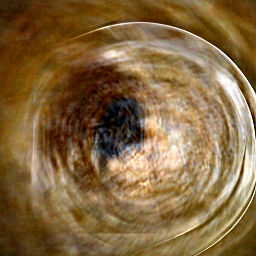
\includegraphics[width=0.158\textwidth]{../fig/unsolved/D4_never_orbit_03_e0.png} & 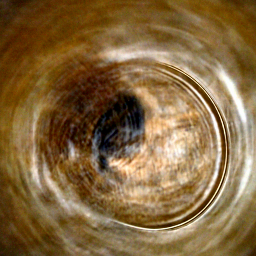
\includegraphics[width=0.158\textwidth]{../fig/unsolved/D4_never_orbit_03_orc.png} & 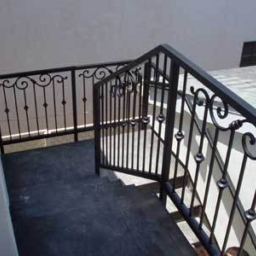
\includegraphics[width=0.158\textwidth]{../fig/unsolved/D4_never_orbit_04_ref.png} & 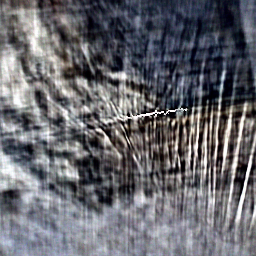
\includegraphics[width=0.158\textwidth]{../fig/unsolved/D4_never_orbit_04_e0.png} & 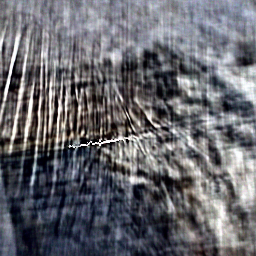
\includegraphics[width=0.158\textwidth]{../fig/unsolved/D4_never_orbit_04_orc.png} \\
ground truth & lowest residual, 17.4\,dB & best, 17.6\,dB, rotated & ground truth & lowest residual, 9.2\,dB & best, 13.8\,dB, rotated \\[3pt]
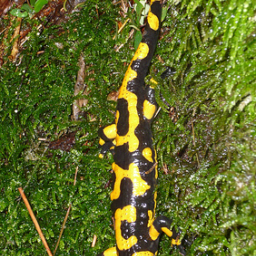
\includegraphics[width=0.158\textwidth]{../fig/unsolved/D4_never_orbit_05_ref.png} & 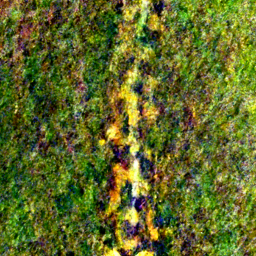
\includegraphics[width=0.158\textwidth]{../fig/unsolved/D4_never_orbit_05_e0.png} & 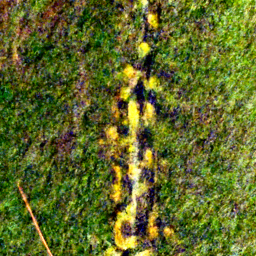
\includegraphics[width=0.158\textwidth]{../fig/unsolved/D4_never_orbit_05_orc.png} & 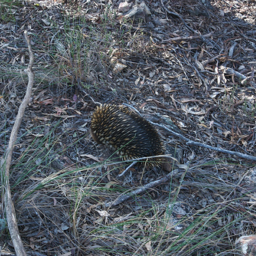
\includegraphics[width=0.158\textwidth]{../fig/unsolved/D4_never_orbit_06_ref.png} & 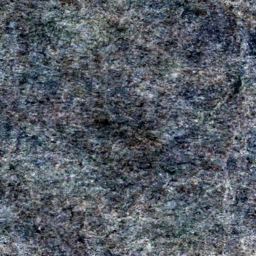
\includegraphics[width=0.158\textwidth]{../fig/unsolved/D4_never_orbit_06_e0.png} & 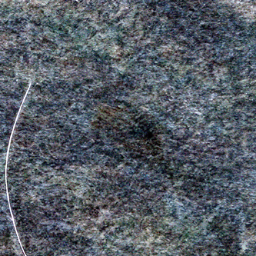
\includegraphics[width=0.158\textwidth]{../fig/unsolved/D4_never_orbit_06_orc.png} \\
ground truth & lowest residual, 14.9\,dB & best, 15.1\,dB & ground truth & lowest residual, 15.3\,dB & best, 16.1\,dB, rotated \\[3pt]
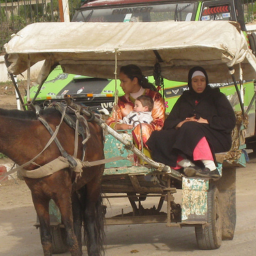
\includegraphics[width=0.158\textwidth]{../fig/unsolved/D4_never_orbit_07_ref.png} & 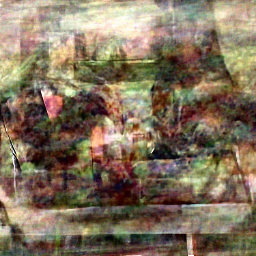
\includegraphics[width=0.158\textwidth]{../fig/unsolved/D4_never_orbit_07_e0.png} & 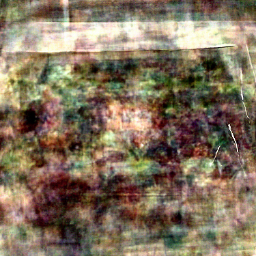
\includegraphics[width=0.158\textwidth]{../fig/unsolved/D4_never_orbit_07_orc.png} & 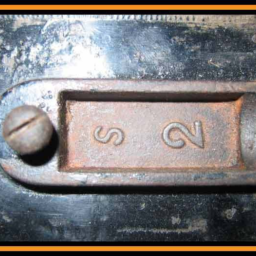
\includegraphics[width=0.158\textwidth]{../fig/unsolved/D4_never_orbit_08_ref.png} & 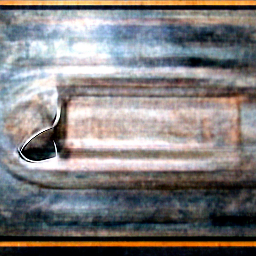
\includegraphics[width=0.158\textwidth]{../fig/unsolved/D4_never_orbit_08_e0.png} & 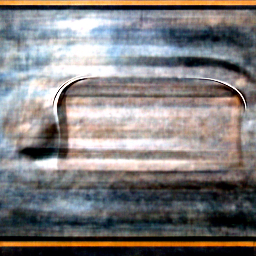
\includegraphics[width=0.158\textwidth]{../fig/unsolved/D4_never_orbit_08_orc.png} \\
ground truth & lowest residual, 12.3\,dB & best, 14.8\,dB & ground truth & lowest residual, 12.0\,dB & best, 12.2\,dB \\[3pt]
\end{tabular}
\caption{\textbf{ImageNet: the first $8$ (by SHA-256 of the image id) of the $22$ images on which FAST-DIPS produces no \good run in any orientation in $64$ runs.} Layout as in \cref{fig:suppl-unsolved-ff}.}
\label{fig:suppl-unsolved-in}
\end{figure}
\clearpage
